% !TEX encoding = UTF-8 Unicode
% !TEX TS-program = pdflatex
% !TEX spellcheck = en-US
% !TEX root = ../Report.tex

\chapter{Optimal Control Design}
Inside this chapter, we are going to show the control system we designed for our application. This phase has been the most complex one for different reasons. Generally speaking, the design of a specific control law for each physical system depends by many factors, having different levels of influence. For this reason, we tried to design the best possible control law by considering more the most important elements and neglecting and/or minimizing the ones with a low impact. As a conseguence, this step required us lots of time to be fully accomplished.\\
At first we ported the system thhat we had theoretically devised into Matlab, initializing all the variables able to influence its behaviour, so that the control could act on a model of a vehicle that was similar to the one used byt the simulator. Then we built the handles to connect with the simulator in order to build simulation environment inside which we could test our control system in comparison with an open loop simulation. Finally, we merged the simulator and the control law together in Simulink and we started optimising the system. \\
\begin{figure}
		\centering
		\lstinputlisting[caption={[SimDataImport]}, firstline=36, lastline=40, firstnumber=36]{../../../model/LinPlant.m}
		\caption{Import vehicle data from the simulator}
		\label{stability}
	\end{figure}
\section{Control Law design}
This step was the most critical one because of its close correlation with the project purpose itself. Our starting object was to develop a control law able to act over the steering angle of the rear wheels, $\delta_{wr}$. We chose to use the Optimal Control Law because that's what we have been presented during the course. In the following paragraphs there will be a brief description of our procedure. In particular, we didn't apply a simple opìtimal control to reduce the erros
\section{Cost Function $J$ Analysis}
Starting from the theory, we studied the real meaning of "Cost Function" and its elements. The function's goal is to design a control system, $u$, ables to minimize the function $J$ itself. In a nutshell, if a certain condition is strongly desired, we have to associate to it a low cost, and viceversa. \\
There follow the linear quadratic form of the cost function $J$ for a general LTI system:
\begin{equation}
J = x^{T}(t_{f}) S_{f} x(t_{f})\int_{t_{0}}^{t_{f}} e^{T} Q e + u^{T} R u \ dt
\end{equation}
where:
\begin{itemize}
	\item $e$ represents a linear combination of \textit{states} x;
	\item $u$ represents the control law;
	\item $ [t_{0},t_{f}] $ represents the time spain in which we evaluated our cost function J;
	\item $ S_{f} = S_{f}^{T} \geq0 $ represents the cost associated to the state once it is evaluated in $t=t_{f}$, so "how much far i am from the origin";
	\item $ Q=Q^{T}\geq 0 $ and $ R=R^{T}\geq 0 $ represent, respectively, the costs for having $e\neq0$ and $u\neq0$, during the time span.
\end{itemize}
\section{Q and R Matrices}
We could reach our final goal, in terms of meaningful imposed rear steering angle, through the "tuning" process of matrices $Q$ and $R$. For what concern the matrix $S$, we set it equal to zero because we didn't need to evaluate the error on the final condition, only during the evolution of the System, so we focused on Q and R matrices. In particular, we started with the rule of thumb of setting the values of these matrices a the inverse of the maximum error we could accept on the states and the inverse of the maximum control we could apply
\begin{equation} \label{Q MAtrix}
	\ Q =
	\begin{bmatrix}
	\ Q_{11} & 0\\
	\ 0 & Q_{22}
	\end{bmatrix} =
	\begin{bmatrix}
	\ inv(max(\beta_{u}-\beta_{u_{ref}})) & 0\\
	\ 0 & inv(max(\omega_{z}-\omega_{f_{ref}}))
	\end{bmatrix}
\end{equation}
\begin{equation} \label{R MAtrix}
	\ R =
	\begin{bmatrix}
	\ R_{11}
	\end{bmatrix} =
	\begin{bmatrix}
	\ inv(max(\delta_{r}))
	\end{bmatrix}
\end{equation}
Q is a diagonal matrix, where $ Q_{11} $ represent the cost of being distant from the equilibrium state of $ \omega_{z} $ and $ Q_{22} $ represents the cost of being distant from the ideal $ \beta_{u} $. $ R_{11} $ instead is relative to the control.
The tuning first steered $ R_{11} $ in order to keep it inside the physical bounds that we decided to set (still tunable, but set 5° in the definitive form), then we modified $ Q_{11} $ and $ Q_{22} $ one in relation with the other, in order to get the best possible compromise.
\section{K multiplier}
Following the theory of optimal control we should extract one single K matrix around the linearization point. This made our working condition very limited, because in choosing a linearization point we would have to choose one single steering angle and angular velocity, thus restricting the range of validity of our system around a certain kind of curve, that initially was as specific as a straight trajectory ($\omega_{z}=0$).
This reason lead us towards the consideration of extracting not one matrix for K, but a whole range of values, based on two inputs from the driver:
\begin{itemize}
	\item front steering angle $\delta_{wf}$
	\item speed $V_0$
\end{itemize}	
This extraction is not done in real time, due to the relatively high computational load of performing an LQR algorithm, it is instead done only once at the startup of the system (now that we are in prototypation phase, later on it will only be performed once and for all). After this initial computations made at some discrete linearization points, the results will be stored in lookup tables, at runtime the only workload for the microcontroller will be to take as input the actual state of the machine, specifically the two input parameters written in the bullet list here above and perform matrix multiplcation as usual.\\
Obviously, given the discrete nature of the lookup table, it will not be possible to have a perfect match for the actual disturbances of the vehicle that span across a continuous space, so we will have to approximate to the nearest point of linearization. It will be anyway a better approximated solution with respect to a system with a single linearization point and a single K.\\
Another reason why we have devoted one script for the extraction of K matrices and another one for the computation of realtime control is that you can't generate C code using matlab coder or even a simulink block with Matlab code containing the lqr algorhytm present in the control system toolbox. We needed to keep it separate.\\
Anyway due to the continuous variation of the equilibrium states, we dont'have big problems on the steep variation of controls.
\begin{figure}[!h]
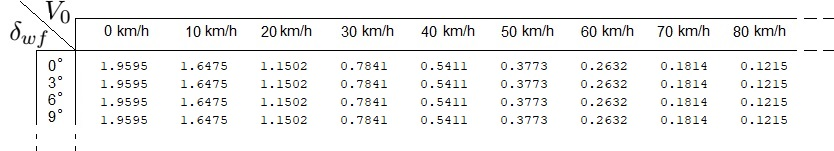
\includegraphics[width=\linewidth]{../Images/KLut.jpg}\caption{Excerpt of K Lookup Table}
\end{figure}
\section{Saturation of control and states}
As we have already written, we saturate the control to a physically feasible range of steering, but this is not enough, because if the results of the lqr algorithm in computing $\omega_{z_{ref}}$ or $\beta_{u_{ref}}$ are out of any phisycally possible range our control will always be saturated, thus not exercising the control that we should expect from it. For this reason we apply a saturation of the states, dependent on the velocity of the vehicle, like the one implemented in the ESP example.
\section{Resulting Control}
\begin{equation} \label{Resulting Control}
	\ \delta_{r} = -
	\begin{bmatrix}
	\ K_{1}\\
	\ K_{2}
	\end{bmatrix}
	\begin{bmatrix}
	\ \beta_{u}-\beta_{u_{ref}} & \omega_{z}-\omega_{z_{ref}}
	\end{bmatrix}
\end{equation}
Where matrix K is obtained from the lookup table generated at startup, while $\omega_{z_{ref}}$ is the result of a real time computation of equilibrium states, $\beta_{u_{ref}}$ instead is set equal to 0 because we want to have the front of the car most aligned possible with the direction of the velocity vector.
